\chapter{Jump Experiment}
\label{app:Jump Experiment}

\begin{table}[!ht]
\centering
\begin{tabular}{l|llll}
\textbf{Frame (no.)} & \textbf{Time (ms)} & \textbf{Height (m)} & \textbf{Interval Velocity (m/s)} & \textbf{Phase}\\
0	&	0	&	0.00000	&	0.000	&	Stance	\\
1	&	84	&	0.05000	&	0.595	&	Decompression launch	\\
2	&	126	&	0.12500	&	1.786	&	Decompression launch	\\
3	&	167	&	0.21250	&	2.134	&	Flight	\\	
4	&	209	&	0.25000	&	0.893	&	Flight + Recovery	\\
5	&	292	&	0.29375	&	0.527	&	Flight + Recovery	\\
6	&	376	&	0.26250	&	-0.372	&	Freefall	\\
7	&	501	&	0.12500	&	-1.100	&	Freefall	\\
8	&	543	&	0.07500	&	-1.190	&	Impact	\\
9	&	584	&	0.00000	&	-1.829	&	Compliant landing	\\
10	&	709	&	0.02500	&	0.200	&	Compliant landing	\\
11	&	793	&	0.04375	&	0.223	&	Compliant landing
\end{tabular}
\caption{Launch and compliant landing video frame data.}
\label{tab:jump-test-data}
\end{table}

\begin{figure}
\centering
\subfloat[][Frame 0.]{
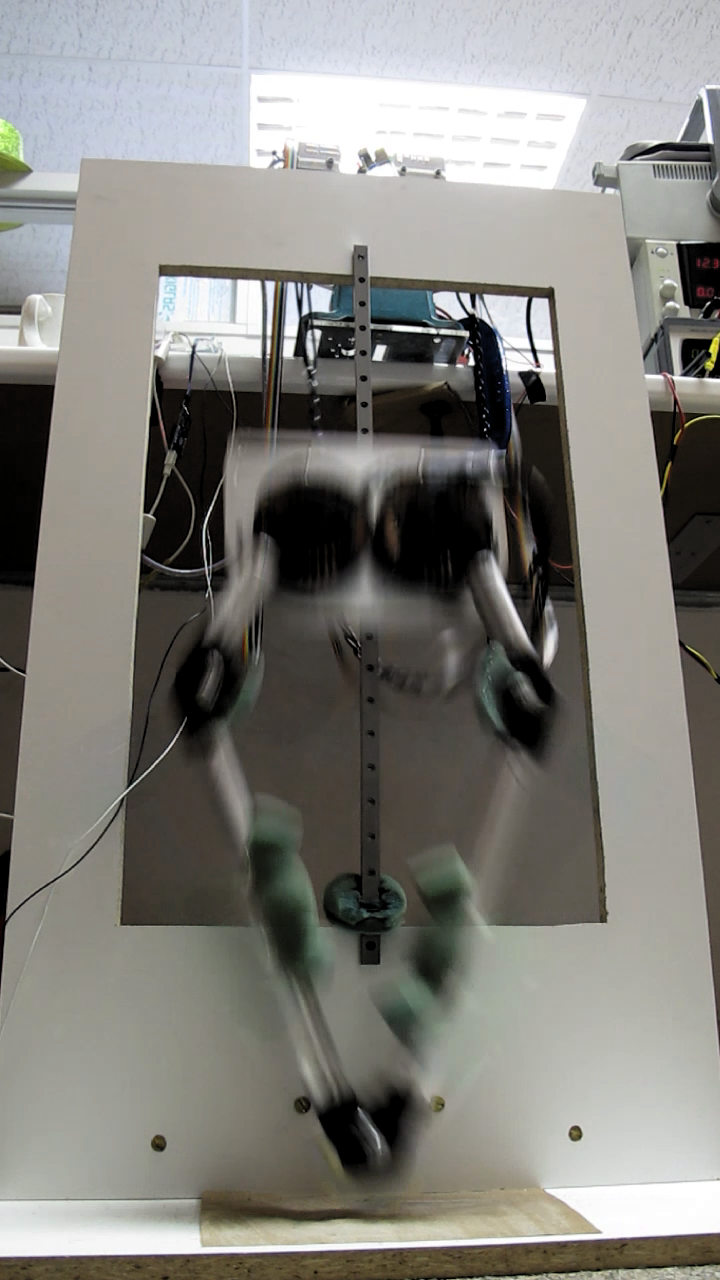
\includegraphics[width=0.3\textwidth]{images/experiments/failed-jump/0.png} 
}
~
\subfloat[][Frame 1: Current cut-out.]{
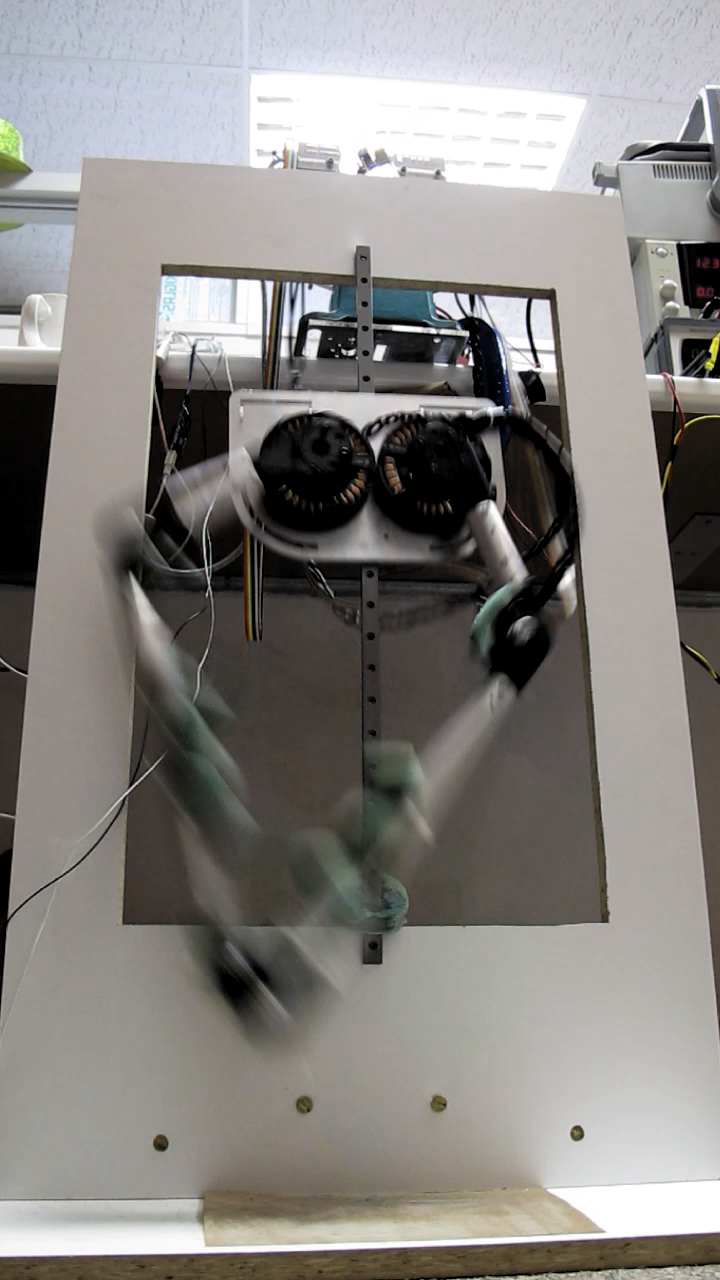
\includegraphics[width=0.3\textwidth]{images/experiments/failed-jump/1.png} 
}
~
\subfloat[][Frame 2.]{
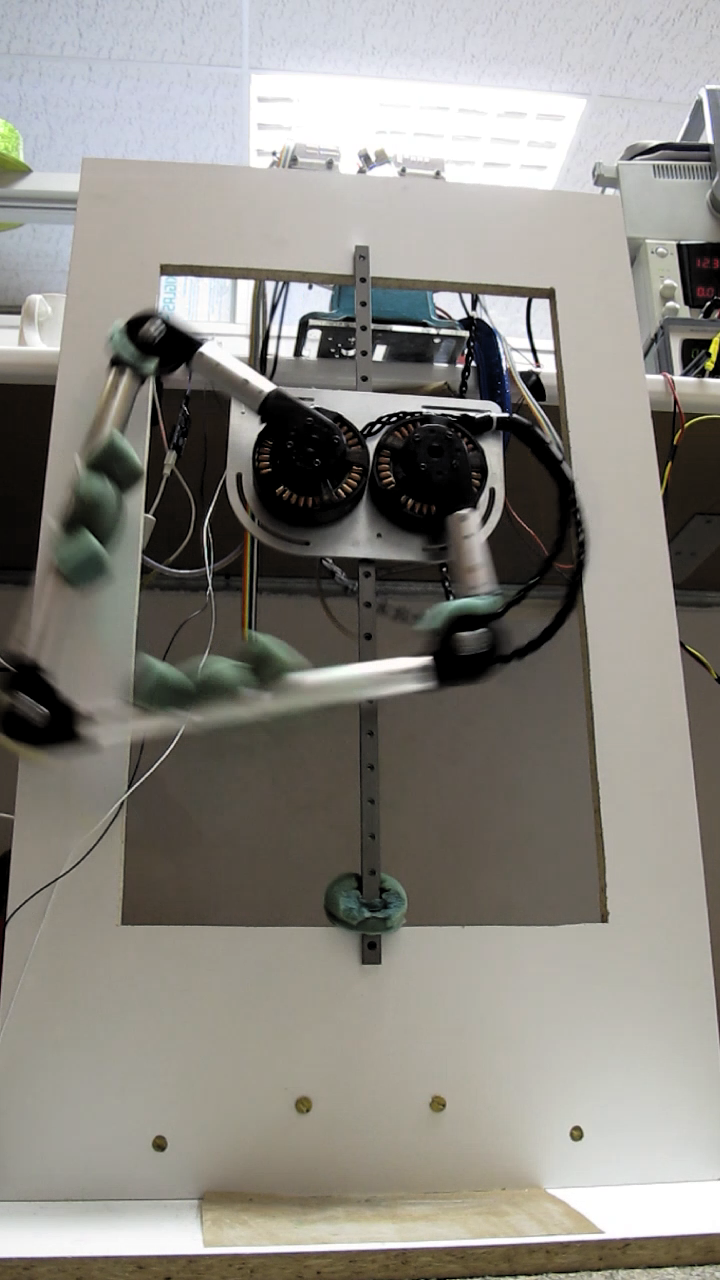
\includegraphics[width=0.3\textwidth]{images/experiments/failed-jump/2.png} 
}

\subfloat[][Frame 3.]{
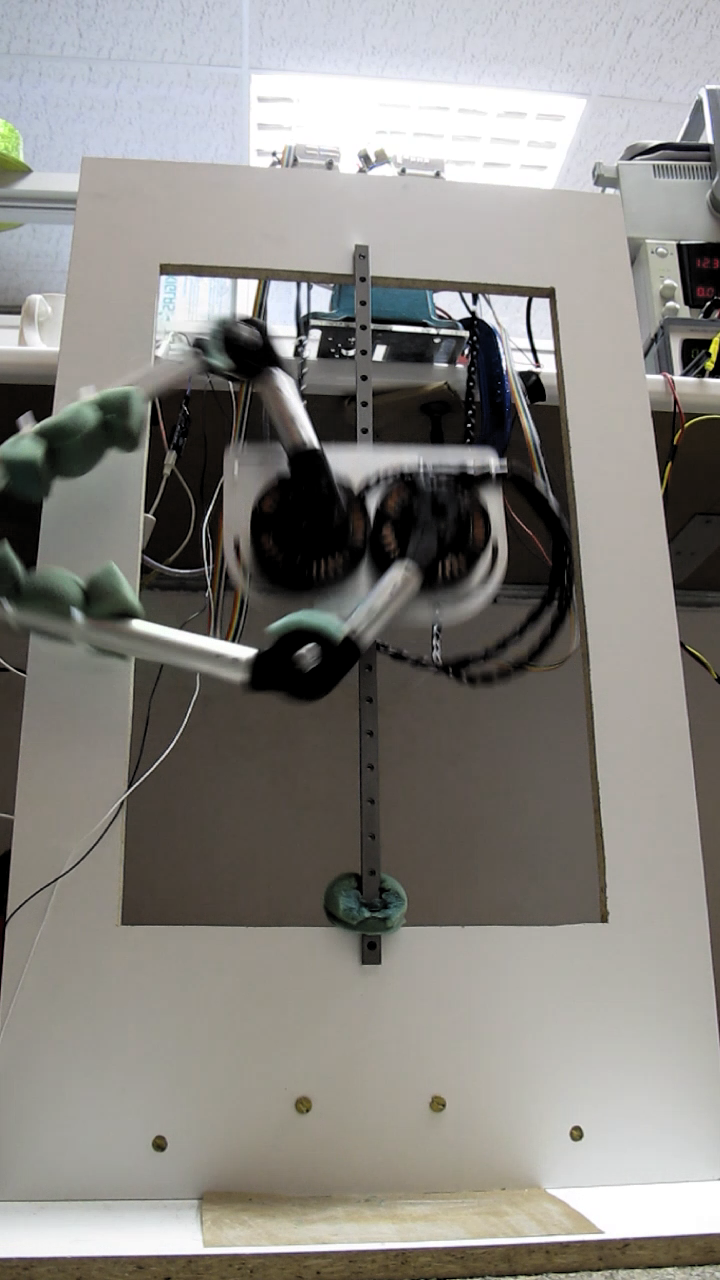
\includegraphics[width=0.3\textwidth]{images/experiments/failed-jump/3.png} 
}
~
\subfloat[][Frame 4.]{
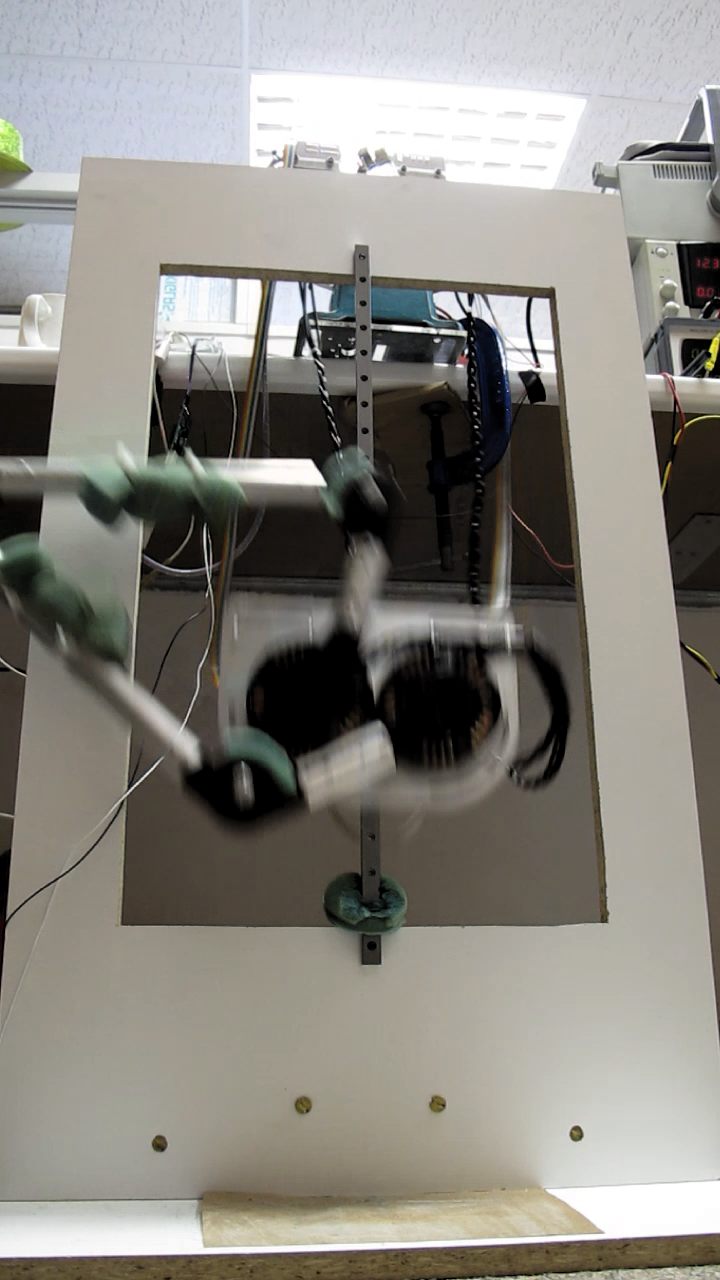
\includegraphics[width=0.3\textwidth]{images/experiments/failed-jump/4.png} 
}
~
\subfloat[][Frame 5.]{
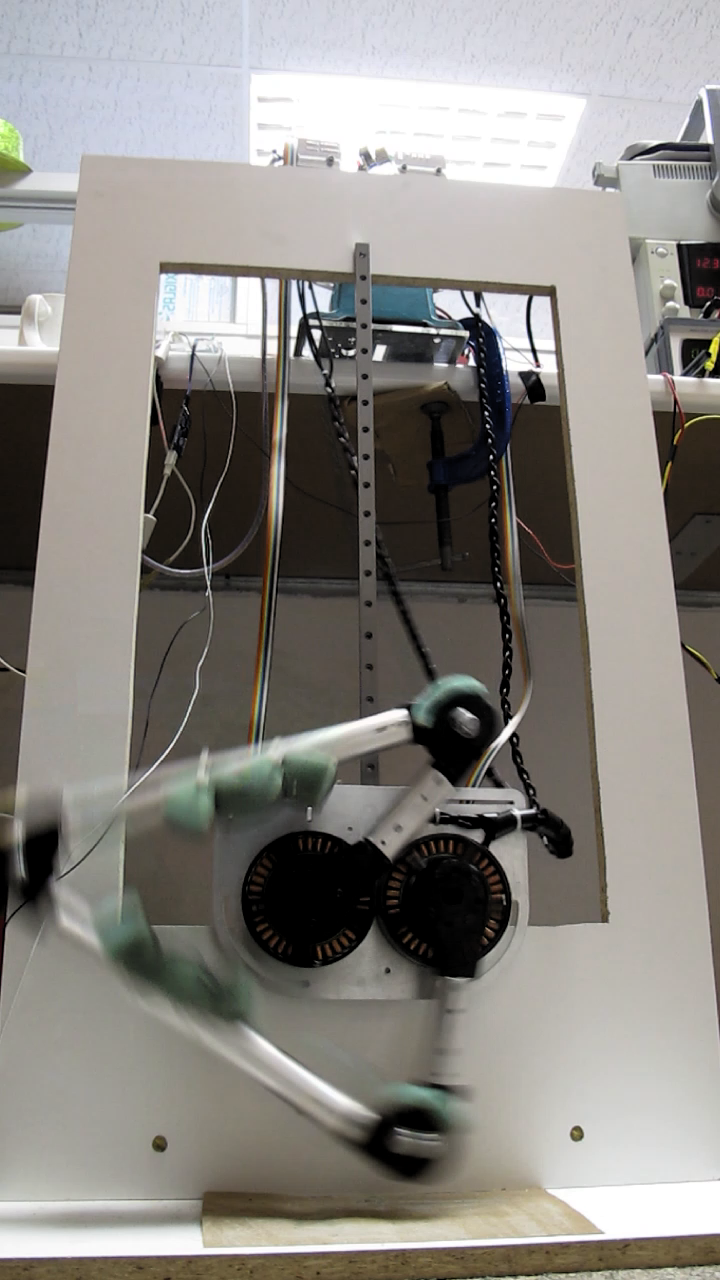
\includegraphics[width=0.3\textwidth]{images/experiments/failed-jump/5.png} 
}
\caption{Motor driver over-current cut-out.}
\label{fig:Motor driver over-current cut-out}
\end{figure}

\begin{listing}[ht]
\begin{minted}[
linenos,
bgcolor=smokyblack]{c}
if(SHOT && r_fbk >= 0.38) {
        r_cmd = 0.3;
        k_r = 1;
        k_s = 0.1;
        ks_r = 633;
        kd_r = 15;
        ks_s = 400;
        kd_s = 5;
        SHOT = 0;
        TRIGGER = 1; //DANGEROUS!
}
if(PULLED && (ELAPSED > 1000)) {
        r_cmd = 0.4;
        k_r = 1;
        k_s = 0.1;
        ks_r = 1726;
        kd_r = 0;
        ks_s = 400;
        kd_s = 5;
        SHOT = 1;
        PULLED = 0;
        ELAPSED = 0;
}
if(TRIGGER) {
        r_cmd = 0.25;
        k_r = 1;
        k_s = 0.1;
        ks_r = 633;
        kd_r = 15;
        ks_s = 400;
        kd_s = 5;
        ELAPSED = 0;
        TRIGGER = 0;
        PULLED = 1;
}
else{
        ELAPSED++;
}
\end{minted}
\caption{Jump control condition loop.}
\label{listing:Jump control condition loop}
\end{listing}